\section{9/3/2019}

\begin{figure}[H]
    \centerline{
        \xymatrix{
            \txt{train \\ $\tilde{p}$} \ar[d] \ar@{<->}[r]^-{D(\tilde{p}, p^*) \leq \eps} \ar[dr]
            & \txt{test\\$p^* \in \cG$} \ar[dr] \\
            \txt{$X_1, \ldots, X_n$\\samples} \ar[r] & 
            \txt{$\hat\theta(\tilde{p})$\\estimator} \ar[r] &
            \txt{$L(p^*, \hat\theta)$\\loss}
        }
    }
    \label{fig:robust-statistics-framework}
    \caption{Overview of the framework. Training distribution $\tilde{p}$ differs
        from test distribution $p^*$ by some discrepancy $D(\tilde{p}, p^*) \leq \epsilon$.
        We constrain $p^* \in \cG$ to encode distributional assumptions.
        Given an estimator $\hat\theta$ trained using samples $X_1, \ldots, X_n \sim \tilde{p}$,
        we want to control the loss $L(p^*, \hat\theta)$ incurred at test time.
    }
\end{figure}


\subsection{Minimum distance functional}

Introduced in \cite{donoho1988automatic}, the minimum distance functional is one way to
produce robust estimators which easily generalizes and also leverages distributional assumptions
in $\cG$.

\begin{definition}[Minimum distance functional]\label{def:mdf}
    The \emph{minimum distance functional} (MDF) is
    \begin{align}
        \hat\theta(\tilde{p}) &= \theta^*(q) = \argmin_{\theta} L(q, \theta)
        \text{ where }
        q = \argmin_{q \in \cG} D(\tilde{p}, q)
    \end{align}
    In other words, $q$ is the projection (under $D$) of $\tilde{p}$ onto $\cG$
    and $\hat\theta$ is the estimator obtained by using $q$ as the training distribution.
\end{definition}

One nice property of the MDF is that we can bound it using a supremum over
nearby pairs $p,q \in \cG$ satisfying $D(p,q) \leq 2 \eps$. This is useful
because we eliminate $\tilde{p}$ and focus the theory around $\cG$.
\begin{proposition}[Modulus of continuity bound]\label{prop:mdf-modulus-error-bound}
    If $D$ is a pseudometric (metric without requirement $d(x,y) = 0 \implies x = y$),
    then the cost $L(p^*, \hat\theta(\tilde{p}))$ of the MDF (\cref{def:mdf}) is bounded by:
    \begin{align}
        \fm(\cG, 2\eps, D, L) &= \sup_{\substack{p, q \in \cG \\ D(p,q) \leq 2 \epsilon}} L(p, \theta^*(q))
    \end{align}
    $\fm$ is called the \emph{modulus of continuity}.
\end{proposition}

\begin{proof}
    First fix $p = p^* \in \cG$
    \begin{align}
        \fm \geq \sup_{g \in \cG : D(p^*, q) \leq 2 \epsilon} L(p^*, \theta^*(g))
    \end{align}
    Next, let $q = \argmin_{g \in \cG} D(g, \tilde{p})$ be the projection of $\tilde{p}$ onto $\cG$
    as in \cref{def:mdf}.
    Then since $D(p^*, \tilde{p}) \leq \eps$ by assumption and $p^* \in \cG$, we have
    \begin{align}
        D(q, \tilde{p}) = \min_{g \in \cG} D(g, \tilde{p}) \leq D(p^*, \tilde{p}) \leq \eps
    \end{align}
    
    The following drawing visualizes the argument.
    \begin{figure}[H]
        \centering
        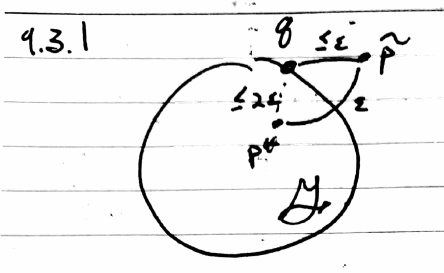
\includegraphics[width=0.7\textwidth]{figures/9-3-1.png}
        \caption{Given $D(p^*, \tilde{p}) \leq \eps$, $p^* \in \cG$, and
            $q$ is the projection of $\tilde{p}$ onto $\cG$ under $D$, we must
            have $D(\tilde{p}, q) \leq \eps$ and by triangle inequality
            $D(p^*, q) \leq 2\eps$
        }
    \end{figure}
    
    So $D(p^*, q) \leq 2 \eps$ and we can conclude
    \begin{align}
        \fm \geq L(p^*, \theta^*(q))
    \end{align}
\end{proof}

For now, we will specialize to the case $D = \TV$ and $L(p,  \theta) = \|\theta - \mu(p^*)\|_2$.
Consider a Gaussian distributional assumption $\cG_{gauss} = \{\cN(\mu, I) : \mu \in \RR^{d}\}$.

\begin{lemma}\label{lem:gauss-tv}
    $\TV(\cN(\mu, I), \cN(\mu', I)) \asymp \Theta(\min(\|\mu - \mu'\|_2, 1))$
    
    Therefore
    \begin{align}
         \fm(\cG_{gauss}, \eps) = \sup_{\substack{p,q \in \cG\\ \TV(p,q) \leq 2 \eps}} \|\mu(p) - \mu(q)\|_2 = \Theta(\eps)   
    \end{align}
    for sufficiently small $\eps$.
\end{lemma}

\begin{proof}
    We first prove the 1D case. By translational symmetry, we can translate both
    distributions while preserving $\|\mu - \mu'\|_2 \eqqcolon u$ so that wlog we may
    assume the two distributions are $p = \cN(\frac{u}{2}, 1)$ and $q = \cN(-\frac{u}{2}, 1)$.
    Then
    \begin{align}
        \TV(p,q)
        &= \frac{1}{2} \frac{1}{\sqrt{2\pi}} \int_{-\infty}^\infty \lvert e^{(t + u/2)^2/2} - e^{(t-u/2)^2/2}\rvert dt \\
        &= \frac{1}{\sqrt{2\pi}} \int_{-u/2}^{u/2} e^{-t^2/2} dt \label{eq:9-3-int}
    \end{align}
    where the last equality follows by cancelling the probability mass in the following picture:
    \begin{figure}[H]
        \centering
        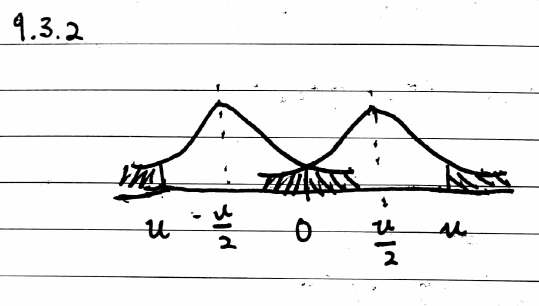
\includegraphics[width=0.7\textwidth]{figures/9-3-2.png}
        \caption{Both Gaussians exhibit identical $\pm \frac{u}{2}$ tails with opposite signs
            in the expression for $\TV$, so the $\TV$ is equivalent to the area in $[-u/2, u/2]$ drawn
            out by the pointwise max between the two PDFs. By symmetry, this is just twice the area
            inside $[-u/2, u/2]$ which after cutting and pasting integration areas (and cancelling the $1/2$
            in definition of $\TV$) is equal
            to the probability mass between $[-u/2,u/2]$ for a Gaussian.}
    \end{figure}
  
    Note that $e^{-t^2/2} \geq \frac{1}{2}$ if $\lvert t \rvert < 1$, so $\TV = \Omega(\min(u,1))$
    which can be seen by splitting the integral and examining the two cases where
    $\frac{u}{2} > 1$ (which yields the $1$) and $\frac{u}{2} < 1$ (which yields the $u$).
    
    Similarly, $e^{-t^2/2} \leq 1$ for all $t > 0$ so $\TV = O(\min(u,1))$.
    
    To generalize to higher dimensions, note identity covariance implies rotational invariance so we can
    rotate and translate such that the two means are on the first coordinate axis and separated
    by $\|\mu - \mu'\| = \lvert \mu_1 - \mu_1' \rvert$. In particular, $\mu_i = 0$ for $i \neq 1$ hence
    in the $\TV$ expression they can be factored out and integrated to $1$ to reduce to the 1D case.
\end{proof}

\subsection{Midpoint lemma and resilience}

As a less restrictive family, consider distributions with bounded covariance:
\begin{align}
    \cG_{cov}(\sigma)
    &= \{ p : \ex_p[(X - u)(X - u)'] \preceq \sigma^2 I\}
\end{align}

We begin with an important lemma which will be used to prove the modulus of continuity for $\cG_{cov}$
and generalized in the following section.
\begin{lemma}\label{lem:midpoint}
    If $\TV(p,q) \leq \eps$ then exists a \emph{midpoint} distribution $r$ such that
    $r \leq \min\{\frac{p}{1 - \eps}, \frac{q}{1 - \eps}\}$ and
    \begin{enumerate}
        \item $r(x) \leq \frac{p(x)}{1 - \eps}$ for all $x$
        \item $r$ is an \emph{$\epsilon$-deletion of $p$} (obtained by deleting $\epsilon$ mass from $p$)
        \item $r = p \vert_{E}$ for $p(E) \geq 1 - \eps$ where $E \mid X$ has probability $1$ if $p(x) \leq q(x)$ and $\frac{q(x)}{p(x)}$ if $p(x) > q(x)$
    \end{enumerate}
\end{lemma}

\begin{proof}
    The midpoint distribution is given by $r = \frac{\min(p,q)}{1 - \TV(p,q)}$ and is obtained from $p$
    by deleting probability mass from $q$ and renormalizing.
    \begin{figure}[H]
        \centering
        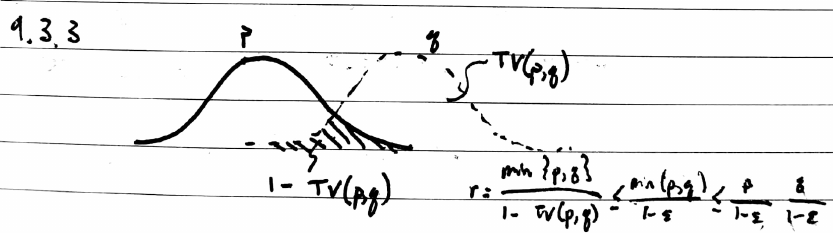
\includegraphics[width=0.6\textwidth]{figures/9-3-3.png}
        \caption{The midpoint distribution $r = \frac{\min(p,q)}{1 - \TV(p,q)}$ can be reached
        from both $p$ and $q$ by deleting $\epsilon$-mass and renormalizing.}
    \end{figure}
    Specifically, we delete
    $q(x) - p(x)$ mass from all points in $\{ x : q(x) > p(x) \}$, the integral of which is precisely
    equal to the total variation distance. This means that we must renormalize by $1 - \eps$ to ensure
    $r$ is a proper distribution.
\end{proof}

\begin{corollary}\label{corr:mod-cont-cov}
    $\fm(\cG_{cov}(\sigma), \eps) = O(\sigma \sqrt{\eps})$
\end{corollary}

\begin{proof}
    Take $p, q \in \cG_{cov}$ such that $\TV(p, q) \leq \eps$.
    By \cref{lem:midpoint}, there exists a midpoint distribution
    $r = p \mid_E$ for which
    \begin{align}
        \ex_r[X - \mu(p)]
        &= \ex_p[X - \mu(p) \mid \underbrace{E}_{1 - \eps}]
        = \frac{-\eps}{1 - \eps} \ex_p[X - \mu(p) \mid \underbrace{E^c}_{\eps}]
    \end{align}
    where the last equality follows from
    \begin{align}
        0
        &= \ex_p[X - \mu(p)]
        = \underbrace{p(E)}_{1-\epsilon} \ex_p[ X - \mu \mid E] + \underbrace{p(E^c)}_{\epsilon} \ex_p[X - \mu \mid E^c]
    \end{align}
    (This is a common trick for moving from conditioning on an event to
    conditioning on its complement in zero mean functionals).
    
    (Chebyshev in $\RR^d$) By linearity of expectation and Jensen's inequality
    \begin{align}
        \| \ex_p[X - \mu(p) \mid E^c] \|_2
        &= \sup_{\|v \|_2 \leq 1} \braket{\ex_p[X - \mu(p) \mid E^c], v} \\
        &= \sup_{\|v\|_2 \leq 1} \ex_p [\braket{X - \mu(p), v} \mid E^c] \\
        &\leq \sup_{\|v \|_2 \leq 1} \sqrt{\ex_p[\braket{X - \mu(p), v}^2 \mid E^c]}
    \end{align}
    Note $\ex_p[\braket{X - \mu(p), v}^2]
    = \Var_p[\braket{X - \mu(p), v}]
    = v^\top \Cov_p(X) v \leq \sigma^2$ so
    \begin{align}
        \| \ex_p[X - \mu(p) \mid E^c] \|_2
        &\leq \sqrt{\frac{\sigma^2}{\Pr[E^c]}}
        = \frac{\sigma}{\sqrt{\eps}}
        \label{eq:9-3-cheb-cov-control}
    \end{align}
    As a result, we have
    \begin{align}
        \|\mu(r) - \mu(p)\|_2 = \|\ex_r[X - \mu(p)]\|_2 \leq \frac{\eps}{1 - \eps} \frac{\sigma}{\sqrt{\eps}} \leq 2 \sigma \sqrt{\eps}
    \end{align}
    for $\eps < 1/2$.
    A similar argument involving $q$ gives $\|\mu(r) - \mu(q)\|_2 \leq 2 \sigma \sqrt{\eps}$
    so by triangle inequality $\|\mu(p) - \mu(q)\|_2 \leq 4 \sigma \sqrt{\eps}$.
\end{proof}

\begin{remark}
    Unlike the trimmed mean, there is no dependence on $d$ here.
    This means that the MDF remains a good robust estimator even in high dimensions!
\end{remark}

The above proof utilizes two key ingredients:
\begin{itemize}
    \item The midpoint property of $\TV$; both $p$ and $q$ are close to some $\eps$-deletion $r$
    \item The bounded tails (second moment) of $\cG_{cov}$, which is used to control how close $\mu(r)$
    and $\mu(p)$ are in \cref{eq:9-3-cheb-cov-control}
\end{itemize}

The previous proof can be suitably generalized to yield a modulus of continuity bound
for other families:
\begin{definition}[Resilient distribution]\label{def:resilience}
    A distribution is $(\rho, \eps)$-resilient if
    \begin{align}\label{eq:resilience-property}
        r \leq \frac{p}{1 - \eps} \implies \|\ex_r[X] - \ex_p[X]\|_2 \leq \rho
    \end{align}
    In other words, for any (not just midpoint) $\eps$-deletion $r$ the mean does not change in
    norm by more than $\rho$. Equivalently (e.g. when $p$ does not have a density) we can view $r = p \mid_E$
    for an event $E$ and use the definition
    \begin{align}
        p(E) \geq 1 - \eps \implies \|\ex_p[X \mid E] - \ex_p[X]\| \leq \rho
    \end{align}
    
    We let $\cG_{TV}(\rho, \epsilon)$ be the set of all $(\rho, \epsilon)$-resilient distributions.
\end{definition}

\begin{remark}
    This definition is only applicable for mean estimation under squared error loss.
\end{remark}

\begin{figure}[H]
    \centering
    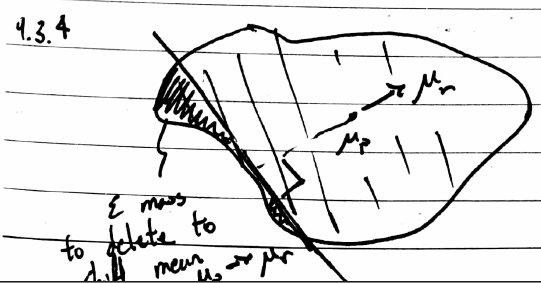
\includegraphics[width=0.5\textwidth]{figures/9-3-4.png}
    \caption{Deleting $\eps$ mass from a resilient distribution $p$ shifts the mean by a controlled
    amount $\|\mu_p - \mu_r\|_2 \leq \rho$.}
\end{figure}

\begin{example}
    \cref{corr:mod-cont-cov} shows $\cG_{cov}(\sigma) \subset \cG_{TV}(2 \sigma \sqrt{\eps}, \eps)$
\end{example}

\begin{example}
    \cref{lem:gauss-tv} shows $\cG_{gauss}(\sigma) \subset \cG_{TV}(\eps \sqrt{\log \frac{1}{\eps}}, \eps)$
\end{example}

Combining with \cref{prop:mdf-modulus-error-bound}, for squared error loss we can say
\begin{corollary}[Modulus of continuity bound for resilient distributions]
    \begin{align}
        \fm(\cG_{TV}(\rho, \eps), \eps) \leq 2 \rho
    \end{align}
\end{corollary}
\begin{proof}
    For any $p,q \in \cG_{\TV}$,
    use \cref{lem:midpoint} to get a midpoint distribution
    and then \cref{eq:resilience-property} with triangle inequality to control the squared error loss.
\end{proof}
So we can always project onto the family of resilient distributions to get a MDF
estimator which has loss independent of $d$.

\subsection{Orlicz norms}

\begin{definition}[Orlitz function / norm]
    An \emph{Orlicz function} $\psi : \RR_{\geq 0} \to \RR_{\geq 0}$ is
    \begin{enumerate}
        \item Convex
        \item Non-decreasing
        \item $\psi(0) = 0$, $\psi(x) \to \infty$ as $x \to \infty$
    \end{enumerate}
    
    Given an Orlicz function $\psi$, the \emph{Orlicz norm} or $\psi$-norm of a
    random variable $X$ is
    \begin{align}
        \|X\|_\psi &= \inf \left\{t : \ex \psi\left(\frac{\lvert X \rvert}{t} \right) \leq 1 \right\}
    \end{align}
    For multivariate $X \in \RR^d$, define 
    \begin{align}
        \|X\|_\psi = \inf \left\{t > 0 : \sup_{v \in \cS^{d-1}} \|\braket{X, v}\|_\psi \leq t \right\}
        \label{def:orlicz-norm-multivar}
    \end{align}
    In other words, $X$ has bounded $\psi$-norm if all of its one dimensional projections do.
    
    Let $\cG_\psi(\sigma) = \{ X : \|X - \ex[X]\|_\psi \leq \sigma \}$.
\end{definition}

\begin{example}
    $\psi(x) = x^k$ gives $\|X\|_\psi = \left(\ex[\lvert X \rvert^k]\right)^{1/k}$,
    which looks like $L_p$ norms. In fact, these are precisely distributions with bounded $k$th moments.
    
    For $\psi(x) = x^2$, we have $\cG_{\psi}(\sigma) = \cG_{cov}(\sigma)$.
\end{example}

\begin{definition}[Sub-Gaussian/Sub-Exponential]\label{def:sub-gaussian-sub-exp-orlicz}
    For $\psi_2(x) = e^{x^2} - 1$, $\cG_{\psi_2}(\sigma)$ are called the $\sigma$-sub-Gaussian random variables.
    
    For $\psi_1(x) = e^x - 1$, $\cG_{\psi_1}(\sigma)$ are called the $\sigma$-sub-exponential random variables.
\end{definition}

The next proposition shows that any distribution with bounded Orlicz norm is resilient.
\begin{proposition}[Bounded Orlicz norm implies resilience]\label{lem:orlicz-norm-resilient}
    $\cG_{\psi}(\sigma) \subset \cG_{TV}(2 \sigma \eps \psi^{-1}(\frac{1}{\eps}), \eps)$
    if $\eps < 1/2$.
    
    $\psi(x) \to \psi^{-1}(x) = \sqrt{x} \to \eps \psi^{-1}(1/\eps) = \sqrt{\eps}$
\end{proposition}

\begin{proof}
    \begin{align}
        \|\ex_r[X] - \ex_p[X]\|_2
        &= \|\ex_p[X - \mu \mid \underbrace{E}_{p(E) = 1 - \eps} ]\|_2
        = \frac{\eps}{1 - \eps} \| \ex_p [ X- \mu \mid E^c] \|
    \end{align}
    Focusing in on the expectation term
    \begin{align}
        \| \ex_p[X - \mu \mid E^c] \|_2
        &= \sup_{\|v\|_2 = 1} \ex_p[\braket{X - \mu, v} \mid E^c]
    \end{align}
    By Jensen's inequality, convexity of $\psi$ (equivalently concavity of $\psi^{-1}$),
    definition of multivariate Orlicz norm (\cref{def:orlicz-norm-multivar}),
    and monotonicity of $\psi$, we have
    \begin{align}
        \| \ex_p[X - \mu \mid E^c] \|_2
        &= \sup_{\|v\|_2 = 1} \sigma \left(
            \ex_p\left[(\sigma \psi^{-1} \circ \psi)\left( \frac{\lvert \braket{X - \mu, v} \rvert}{\sigma} \right) \mid E^c\right]
        \right) \\
        &\leq \sup_{\|v\|_2 = 1} \sigma \psi^{-1}\left(
            \ex_p\left[\psi\left( \frac{\lvert \braket{X - \mu, v} \rvert}{\sigma} \right) \mid E^c\right]
        \right) \\
        &\leq \sup_{\|v\|_2 = 1} \sigma \psi^{-1}\left(
            \underbrace{\ex_p\left[\psi\left( \frac{\lvert \braket{X - \mu, v} \rvert}{\sigma} \right) \right]}_{\leq 1}
            \underbrace{\frac{1}{\Pr[E^c]}}_{\frac{1}{\eps}}
        \right) \\
        &\leq \sigma \psi^{-1}(\frac{1}{\eps})
    \end{align}
\end{proof}